\documentclass[12pt,a4paper]{article}
\usepackage{ctex}
\usepackage{amsmath,amscd,amsbsy,amssymb,latexsym,url,bm,amsthm}
\usepackage{epsfig,graphicx,subfigure}
\usepackage{enumitem,balance}
\usepackage{wrapfig}
\usepackage{mathrsfs,euscript}
\usepackage[usenames]{xcolor}
\usepackage{hyperref}
\usepackage{appendix}
\usepackage{soul}
\usepackage{listings}
\usepackage[vlined,ruled,linesnumbered]{algorithm2e}
\usepackage{array}
\hypersetup{colorlinks=true,linkcolor=black}

\newtheorem{theorem}{Theorem}
\newtheorem{lemma}[theorem]{Lemma}
\newtheorem{proposition}[theorem]{Proposition}
\newtheorem{corollary}[theorem]{Corollary}
\newtheorem{exercise}{Exercise}
\newtheorem*{solution}{Solution}
\newtheorem{definition}{Definition}
\theoremstyle{definition}

\renewcommand{\thefootnote}{\fnsymbol{footnote}}

\newcommand{\postscript}[2]
 {\setlength{\epsfxsize}{#2\hsize}
  \centerline{\epsfbox{#1}}}

\renewcommand{\baselinestretch}{1.0}

\setlength{\oddsidemargin}{-0.365in}
\setlength{\evensidemargin}{-0.365in}
\setlength{\topmargin}{-0.3in}
\setlength{\headheight}{0in}
\setlength{\headsep}{0in}
\setlength{\textheight}{10.1in}
\setlength{\textwidth}{7in}
\makeatletter \renewenvironment{proof}[1][Proof] {\par\pushQED{\qed}\normalfont\topsep6\p@\@plus6\p@\relax\trivlist\item[\hskip\labelsep\bfseries#1\@addpunct{.}]\ignorespaces}{\popQED\endtrivlist\@endpefalse} \makeatother
\makeatletter
\renewenvironment{solution}[1][Solution] {\par\pushQED{\qed}\normalfont\topsep6\p@\@plus6\p@\relax\trivlist\item[\hskip\labelsep\bfseries#1\@addpunct{.}]\ignorespaces}{\popQED\endtrivlist\@endpefalse} \makeatother

\begin{document}
\noindent

%========================================================================
\noindent\framebox[\linewidth]{\shortstack[c]{
\Large{\textbf{Lab08-Graph Exploration}}\vspace{1mm}\\
CS214-Algorithm and Complexity, Xiaofeng Gao \& Lei Wang, Spring 2021.}}
\begin{center}
\footnotesize{\color{blue}$*$ Name:\underline{\quad   Haoyi You  \quad  }\quad Student ID:\underline{\quad 519030910193 \quad} \quad Email: \underline{\quad yuri-you@sjtu.edu.cn \quad}}
\end{center}

\begin{enumerate}

	\item Given an undirected graph $G = (V, E)$. Prove the following propositions.
	
	\begin{enumerate}
		\item Let $e$ be a maximum-weight edge on some cycle of connected graph $G=(V,E)$.
        Then there is a minimum spanning tree of $G$ that does not include $e$. Moreover, there is no minimum spanning tree of $G$ that includes $e$ if $e$ is the unique maximum-weight edge on the cycle. 
		\item Let $T$ and $T'$ are two different minimum spanning trees of $G$. Then $T'$ can be obtained from $T$ by repeatedly substitute one edge in $T\backslash T'$ by one edge in $T'\backslash T$ and meanwhile the result after each substitution is still a minimum spanning tree.
	\end{enumerate}
	\begin{solution}
	~\par
	\begin{enumerate}
	    \item 
	    ~\par
	    Assume $T$ is a minimum spanning tree of $G$ that include $e$, and $e=(u,v)$ .So $u,v$ is not connected in $T\backslash\{e\}$. \\There also exists another edge $e'=(u',v')$ in an cycle together with $e$ that $e'\notin T$, otherwise the whole cycle is belonged to $T$, which is against with $T$ is a tree. \\In $T\backslash\{e\}$, $u$ is connected with either $u'$ or $v'$, so assume $u$ is connected to $u'$. Since $T$ is a spanning tree but $T\backslash\{e\}$ is not, $v$ is connected with $v'$.\\
	    If $e$ is a maximum-weight edge on the cycle, the new tree $T'=T\backslash\{e\}\cap\{e'\}$ is also a spanning tree, and $w(T)\ge w(T')$. So $T'$ is also a minimum spanning tree with $e \notin T'$.\\
	    If  $e$ is the unique maximum-weight edge on the cycle, $w(T)>w(T')$,which is against with the assumption that $T$ is a minimum spanning tree of $G$.So there is no minimum spanning tree of $G$ includes $e$.
	    \item
	    Firstly, since $T$ and $T'$ are both spanning tree, $|T|=|T'|$, so $|T-T'|=|T'-T|=x$, which means we can take $x$ substitution operation to change the $|T|$ to $|T'|$.\\
	    Secondly, we prove after every substitution operation, the result is also a spanning tree.\\
	    $\forall$ choose an edge $e\in T-T'$, the graph $T$ is connected but $T\backslash\{e\}$ is not connected. So we can find a partition of two parts $V_1$ and $V_2$ of all the vertices in $G$, that vertices in $V_1$ or $V_2$ are connected but $\forall v_1\in V_1,v_2\in V_2,v_1~v_2$ is not connected.\\
	    There must exist an edge $e'=(u,v)$ in $T'$ that $u\in V_1$ and $v\in V_2$. Since $e\notin  T'\leftarrow e\notin T'\cap T$, so in $T\cap T', V_1~V_2$ is not connected. However, $T'$ is connected, so $e'\in T'-(T\cap T')=T-T'$.\\
	    As a result, in $T\backslash\{e\}\cup \{e'\}$ ,$V_1$ and $V_2$ is connected. So $T\backslash\{e\}\cup \{e'\}$ is a spanning tree after substituting $e$ by $e'$ in $T$.\\
	    Let $T=T\backslash\{e\}\cup \{e'\}$ and recursively use the operation above,then we substitute $T$ by $T'$ and all the results in the process are all spanning tree.\\
	    Thirdly, if we guarantee the $e$ be the maximum weight in $T-T'$,then all the spanning tree are all minimum-weighted,which means $w(e)=w(e')$.\\
	    If $w(e)>w(e')$,the weight of result is smaller, which is against with the $T$ is a minimum spanning tree.\\
	    If $w(e)<w(e')$, $\forall e_0\in T-T', w(e_0)<w(e')$. So we reverse the process, change $T'$ to $T$, and choose the $e'$ be substitute at the first time, then there exists $e_1
	    \in T-T'$, the $T'\backslash\{e'\}\cup\{e_1\}$ is also a spanning tree, but obviously the weight of $T'\backslash\{e'\}\cup\{e_1\}$ is smaller than $T'$, which is against with $T'$ is a minimum-weight spanning tree.
	\end{enumerate}
	\end{solution}
    \item Let $G=(V,E)$ be a connected, undirected graph. Give an $O(|V|+|E|)$-time algorithm
    to compute a path in $G$ that traverses each edge in $E$ exactly once in each direction. Describe how you can find your way out of a maze if you are given enough coins to apply your algorithm.
    \begin{solution}
    ~\par
    	\begin{algorithm}[H]
		\KwIn{A Graph $G=(V,E)$}
		\KwOut{A Path of Edge Queue $Q$}
		
		\BlankLine
		\caption{Find Euler Road}\label{Alg-quicksort}
		$Odd\_Node\leftarrow 0;$\\
		\For{$v \in V$}{
			\If{$d(v)\%2==1$}{
				$Odd\_Node\leftarrow Odd\_Node+1$;\\
				$Now\_Node\leftarrow v$;
			}
		}
		\If{$Odd\_Node>2$}{
		    throw error "do not exist such path";\\
		    \Return;
		}
		$Q\leftarrow$ NULL;\\
		\While{$V$ is not empty}{
		    find $(Now\_Node,v) \in E$;\\
		    $Q.push((Now\_Node,v))$;\\
		    Delete $(Now\_Node,v)$ in graph $G$;\\
		    $Now\_Node\leftarrow v;$\\
		}
		\Return Q;
	\end{algorithm}
    \end{solution}
    \item Consider the maze shown in Figure \ref{Fig-Maze}. The black blocks in the figure are blocks that can not be passed through. Suppose the block are explored in the order of right, down, left and up. That is, to go to the next block from $(X,Y)$, we always explore $(X,Y+1)$ first, and then $(X+1,Y)$,$(X,Y-1)$ and$(X-1,Y)$ at last. Answer the following subquestions:
    \begin{enumerate}
        \item Give the sequence of the blocks explored by using DFS to find a path from the "start" to the "finish".
        \item Give the sequence of the blocks explored by using BFS to find the \underline{shortest} path from the "start" to the "finish".
        \item Consider a maze with a larger size. Discuss which of BFS and DFS will be used to find one path and which will be used to find the shortest path from the start block to the finish block.
    \end{enumerate}
    \begin{solution}
    ~\par
    \begin{enumerate}
        \item DFS:$(A,A)\rightarrow(B,A)\rightarrow(B,B)\rightarrow(B,C)\rightarrow(C,C)\rightarrow(B,C)\rightarrow(A,C)\rightarrow(A,D)\rightarrow(A,E)\rightarrow(B,E)\rightarrow(C,E)\rightarrow(D,E)\rightarrow(D,D)$.
        \item BFS:$(A,A)\rightarrow(B,A)\rightarrow(B,B)\rightarrow(C,A)\rightarrow(B,C)\rightarrow(D,A)\rightarrow(C,C)\rightarrow(A,C)\rightarrow(D,B)\rightarrow(A,D)\rightarrow(E,B)\rightarrow(A,E)\rightarrow(E,C)\rightarrow(B,E)\rightarrow(E,D)\rightarrow(C,E)\rightarrow(D,D)$.\\
        The shortest path is $(A,A)\rightarrow(B,A)\rightarrow(C,A)\rightarrow(D,A)\rightarrow(D,B)\rightarrow(E,B)\rightarrow(E,C)\rightarrow(E,D)\rightarrow(D,D)$.
        \item If we only want to find a path, DFS and BFS are both ok, but the effect of DFS is better, for DFS wants to explore more deeper until find dead end, but BFS is to explore all the possible ways, which must take a lot of time.\\
        However, if we want to find shortest path, we can only use BFS. In one round of exploration, each block explored is the same distance from the start. So the first time we explore the destination will be the shortest path. 
    \end{enumerate}
    \end{solution}
    \begin{figure}[!htbp]
	\centering
	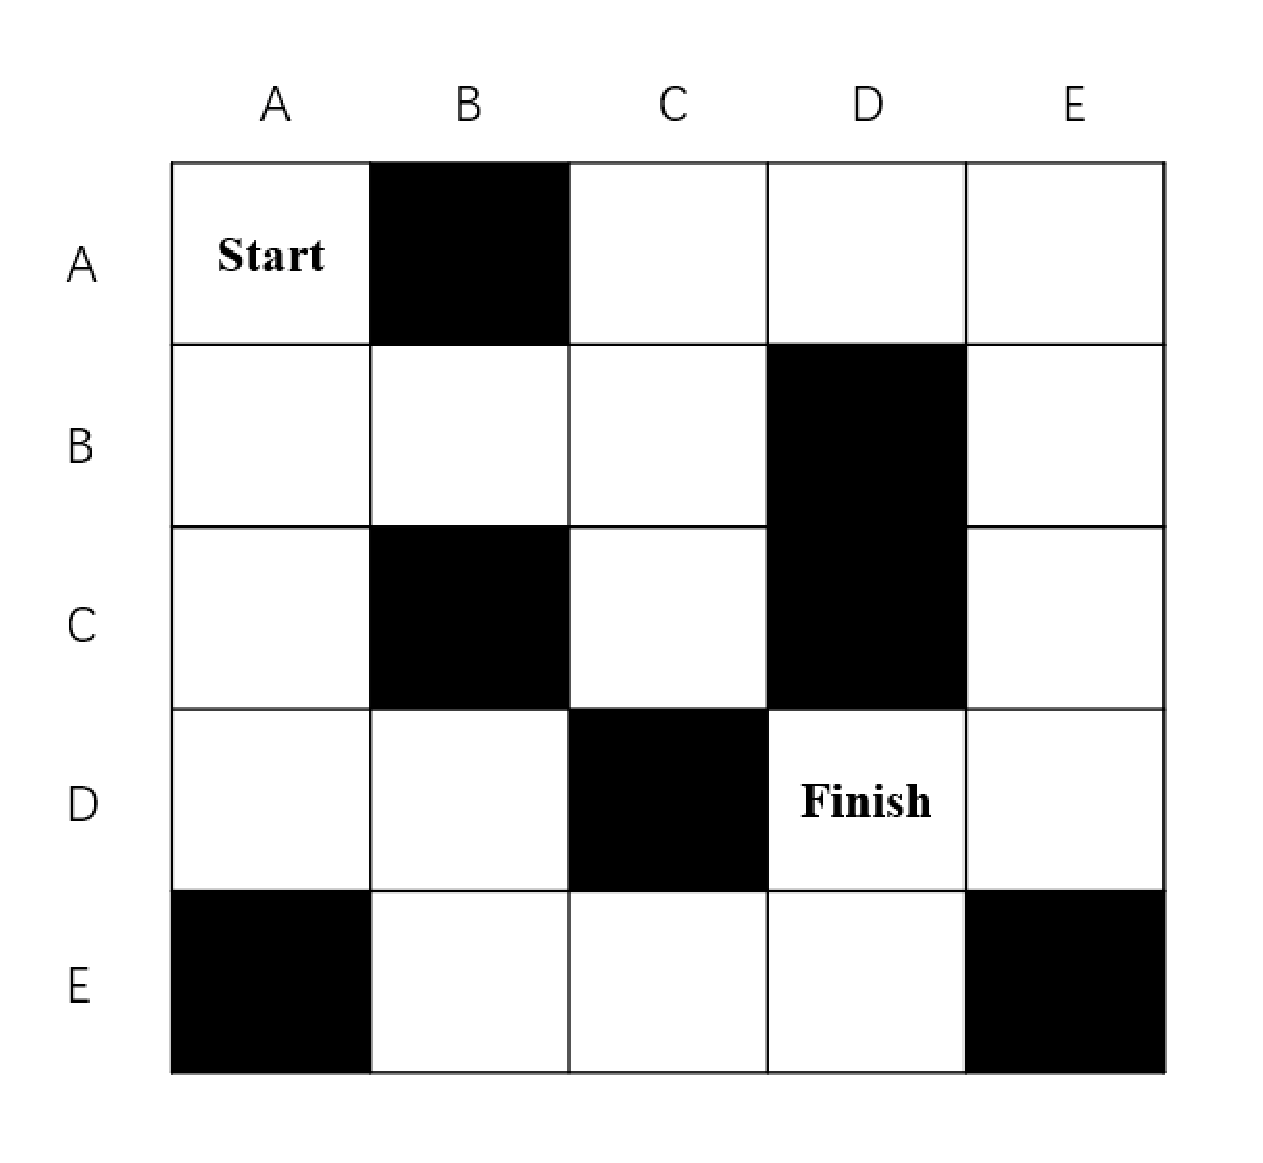
\includegraphics[width=0.45\textwidth]{Fig-Maze.pdf}
	\caption{The blocks in the maze.}
	\label{Fig-Maze}
	\end{figure}
	
	\item Given a directed graph $G$, whose vertices and edges information are introduced in data file "SCC.in". Please find its number of Strongly Connected Components with respect to the following subquestions.
    
    \begin{enumerate}
    	\item Read the code and explanations of the provided C/C++ source code "SCC.cpp", and try to complete this implementation.
    	\item Visualize the above selected Strongly Connected Components for this graph $G$. Use the $Gephi$ or other software you preferred to draw the graph. {\color{blue}(If you feel that the data provided in ``SCC.in'' is not beautiful, you can also generate your own data with more vertices and edges than $G$ and draw an additional graph. Notice that results of your visualization will be taken into the consideration of Best Lab.)}
    \end{enumerate}	
    \begin{solution}
    ~\par
    \begin{enumerate}
        \item The result is 202.\\
        Here we provide two algorithm code. The tarjan algorithm is in appendix 1. The kosaraju algorithm is in appendix 2.
        \item Using the origin data we can get the result figure ~\ref{result1}.
        \begin{figure}[htbp]
        \centering
        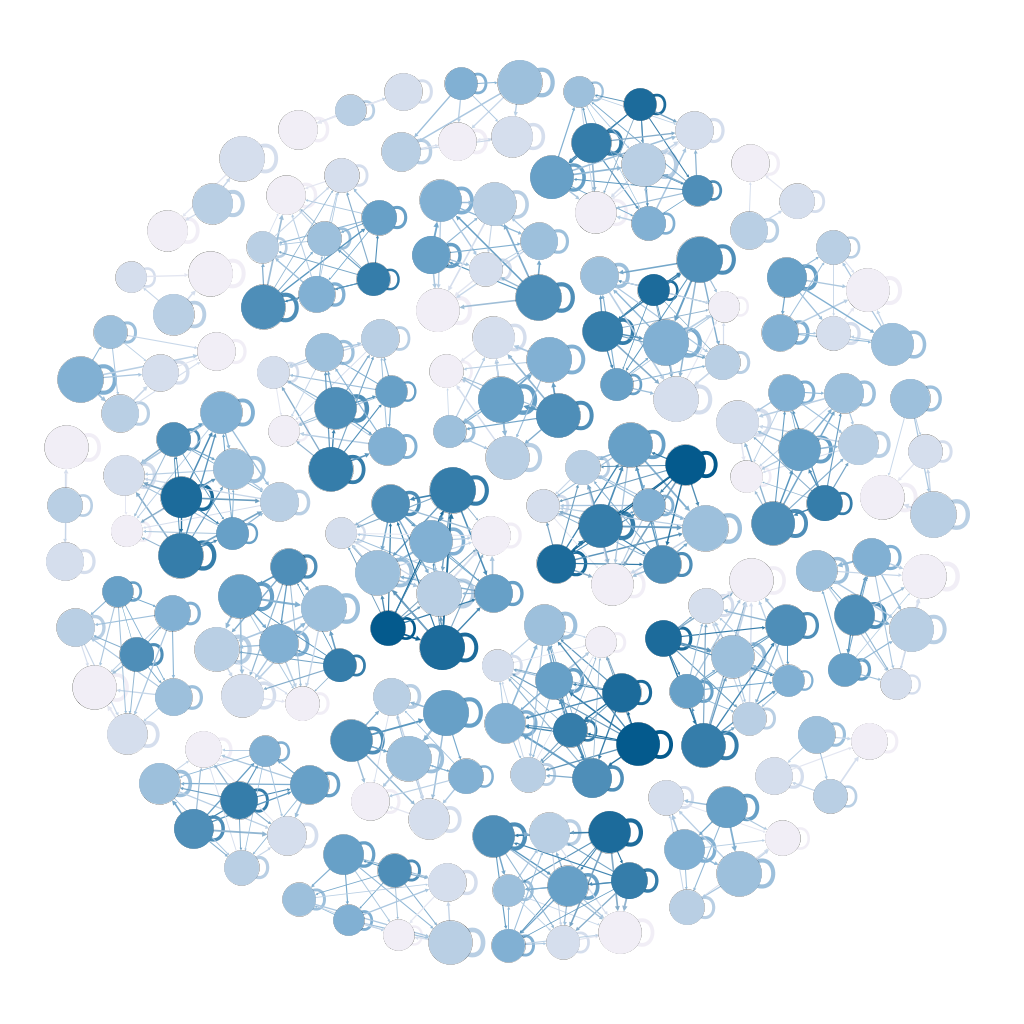
\includegraphics[width=0.4\textwidth]{result.png}
        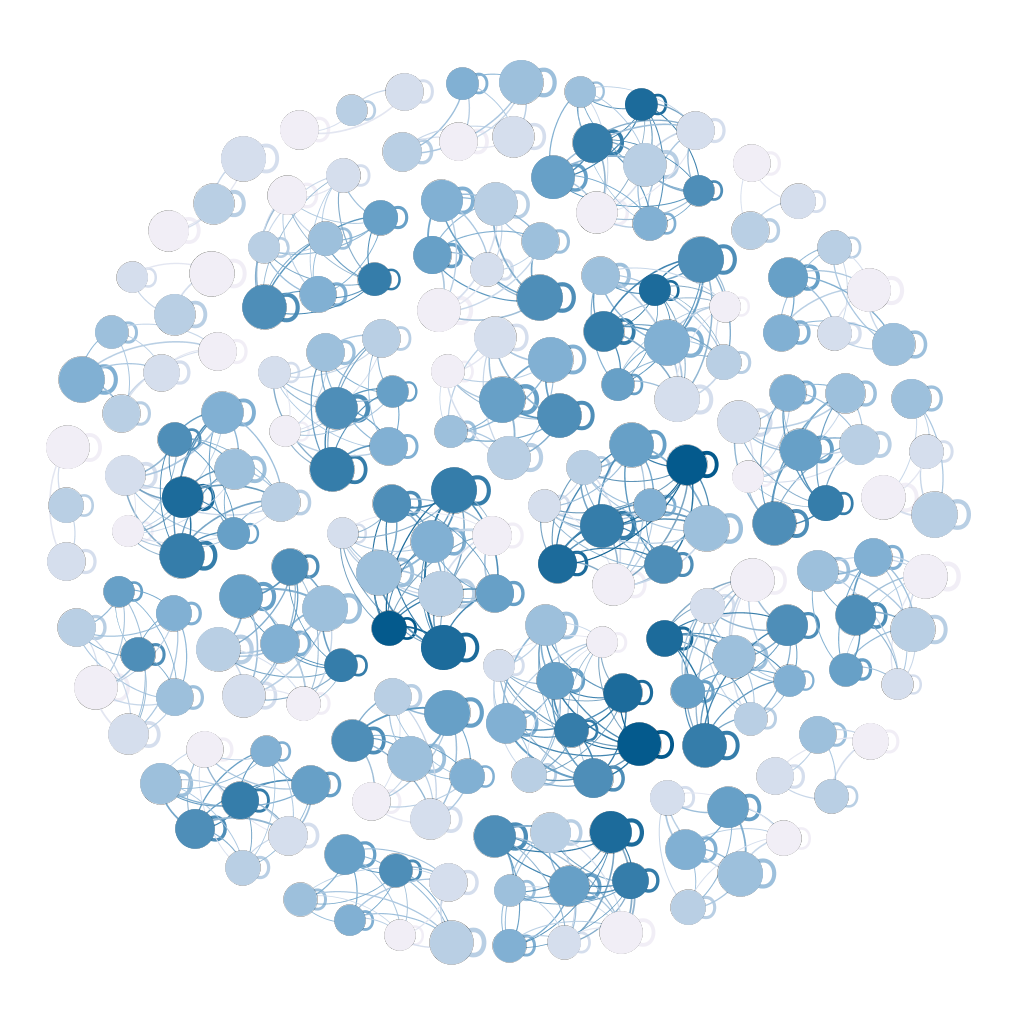
\includegraphics[width=0.4\textwidth]{result_curve.png}
        \caption{SCC in graph}\label{result1}
        \end{figure} 
        But if I dispose the data in a cpp program based on the above program, we can get a much more tidy figure ~\ref{result2}
        \begin{figure}[htbp]
        \centering
        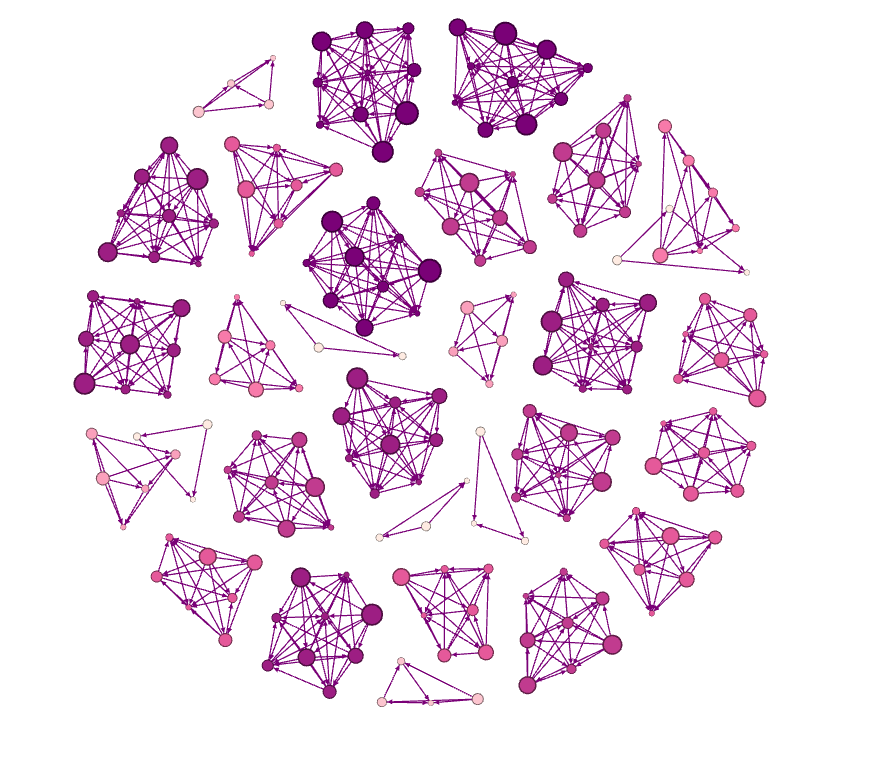
\includegraphics[width=0.8\textwidth]{modify.png}
        \caption{Disposed data of SCC in graph}\label{result2}
        \end{figure} 
        \par It is necessary to mention that every vertex in graph represents a strongly connected component in graph, and the size of it shows the number of vertex in this connected component.
    \end{enumerate}
    \end{solution}
\end{enumerate} 

\section{Appendix1}
\begin{lstlisting}[language=C++]
#include <vector>
#include <iostream>
#include <fstream>
#include <stack>
using namespace std;
int mins(int a, int b) {
    return (a < b) ? a : b;
}
int Search(vector<vector<int>>& graph,int* DFN,int* LOW,int vetex,
int& time,int& ans,stack<int>& s,bool* in_stack) {
    ++time;
    in_stack[vetex] = true;
    s.push(vetex);
    DFN[vetex] = LOW[vetex]=time;
    int get_low;
    for (int k : graph[vetex]) {
        if (DFN[k]!=0) {// have explored
            if (in_stack[k])
                LOW[vetex] = mins(LOW[k], LOW[vetex]);
        }
        else{//haven't explored
            Search(graph, DFN, LOW, k, time, ans,s,in_stack);
            LOW[vetex] = mins(LOW[vetex], LOW[k]);
        }
    }
    if (DFN[vetex] == LOW[vetex]) {//vetex and its subtree is a SCC
        ++ans;//The number of SCC increases
        int pop_node=s.top();
        in_stack[pop_node] = false;
        while (pop_node != vetex) {
            s.pop();
            pop_node = s.top();
            in_stack[pop_node] = false;
        }
        s.pop();//Pop this tree in the stack
    }
    return LOW[vetex];
}
int SCC(int n, vector<pair<int,int>>& edge) {
    vector<vector<int>> graph;
    for (int i = 0; i < n; ++i) {
        graph.push_back(vector<int>());
    }
    for (pair<int,int> t : edge) {
        graph[t.first].push_back(t.second);
    }//change to the adjacency list
    int* DFN = new int[n];//The time explore the n
    int* LOW = new int[n];//The minimum time explore the n or its subtree
    bool* in_stack= new bool[n];
    memset(DFN, 0, n * sizeof(n));
    memset(in_stack, 0, (n) * sizeof(bool));
    int now = 0;
    int ans = 0;
    int time = 0;
    stack<int> s;
    while (now <n) {
        if (DFN[now]==0) {
            Search(graph,DFN, LOW, now, time,ans,s,in_stack);
        }
        ++now;
    }
    delete[] DFN;
    delete[] LOW;
    delete[] in_stack;
    return ans;
}
//Please do NOT modify anything in main(). Thanks!
int main()
{
    int m,n;
    vector<pair<int,int>> edge;
    ifstream fin;
    ofstream fout;
    fin.open("SCC.in");
    cout<<fin.is_open()<<endl;
    fin>>n>>m;
    cout<<n<<" "<<m<<endl;
    int tmp1,tmp2;
    for(int i=0;i<m;i++)
    {
        fin>>tmp1>>tmp2;
        edge.push_back(pair<int,int>(tmp1,tmp2));
    }
    fin.close();
    int ans=SCC(n,edge);
    fout.open("SCC.out");
    fout<<ans<<'\n';
    cout << ans;
    fout.close();
    return 0;
}

\end{lstlisting}
\section{Appendix2}
\begin{lstlisting}[language=C++]
#include <vector>
#include <iostream>
#include <fstream>
#include <queue>
#include <stack>
using namespace std;
stack<int> s;
struct vertex {
    bool explore, explore2;
    vertex() :explore(false),explore2(false) {}
};
void DFS1(vector<vector<int>>& graph, vertex* v,int vertex) {
    v[vertex].explore = true;
    for (auto k : graph[vertex]) {
        if (!v[k].explore) {
            DFS1(graph, v, k);
        }
    }
    s.push(vertex);
}
void DFS2(vector<vector<int>>& graph, vertex* v, int vertex) {
    v[vertex].explore2 = true;
    for (auto k : graph[vertex]) {
        if (!v[k].explore2) {
            DFS2(graph, v, k);
        }
    }
}
int SCC(int n, vector<pair<int,int>>& edge) {
    vector<vector<int>> graph;
    vector<vector<int>> anti_graph;
    for (int i = 0; i < n; ++i) {
        graph.push_back(vector<int>());
        anti_graph.push_back(vector<int>());
    }
    for (pair<int,int> t : edge) {
        graph[t.first].push_back(t.second);
        anti_graph[t.second].push_back(t.first);
    }//change to the adjacency list
    vertex* v = new vertex[n];
    int now = 0;
    int ans = 0;
    while (now < n) {
        if (!v[now].explore) {
            DFS1(anti_graph,v,now);
        }
        ++now;
    }
    while (!s.empty()) {
        int v1 = s.top();
        s.pop();
        if (!(v[v1].explore2)) {
            DFS2(graph, v, v1);
            ++ans;
        }
    }
    delete[]v;
    return ans;
}
//Please do NOT modify anything in main(). Thanks!
int main()
{
    int m,n;
    vector<pair<int,int>> edge,another;
    ifstream fin;
    ofstream fout;
    fin.open("SCC.in");
    cout<<fin.is_open()<<endl;
    fin>>n>>m;
    cout<<n<<" "<<m<<endl;
    int tmp1,tmp2;
    for(int i=0;i<m;i++)
    {
        fin>>tmp1>>tmp2;
        edge.push_back(pair<int,int>(tmp1,tmp2));
    }
    fin.close();
    int ans=SCC(n,edge);
    fout.open("SCC.out");
    fout<<ans<<'\n';
    cout << ans;
    fout.close();
    return 0;
}

\end{lstlisting}


\newpage


%========================================================================
\end{document}